\newpage
%%%%%%%%%%%%%%%%%%%%%%%%%%%%%%%%%%%%%%%%%%%%%%%%%%%%%%%%%%%%%%%%%%%%%%%%%%%%%%%%
%%%%%%%%%%%%%%%%%%%%%%%%%%%%%%%%%%%%%%%%%%%%%%%%%%%%%%%%%%%%%%%%%%%%%%%%%%%%%%%%
\section{Princípios elementares e gerais na dança de salão}
\label{sec:PrincipioGeral}
\index{Princípios elementares!Dança de salão}


\begin{tcbattention}
É importante aclarar
que os princípios elementares expostos neste capítulo e posteriores, 
não estão regulamentadas por nenhuma entidade ou instituição; assim, 
estes princípios refletem, o meu aprendizado de distintos professores,
interpretações pessoais  e deduções. 
\end{tcbattention}

Neste capítulo veremos um conjunto de \hyperref[def:Principio]{\textbf{princípios elementares}}, 
e a explicação de como o cumprimento ou não destes, 
afetam ao desenvolvimento estético e técnico da \hyperref[def:DancaSalao]{\textbf{dança de 
salão}}\footnote{Ou na \hyperref[def:DancaSocial]{\textbf{dança social}} sim se está interessado em levar estas ideias a esse âmbito.}  no \hyperref[def:ParadigmaConducao]{\textbf{paradigma da condução}}.

Os \hyperref[def:Principio]{\textbf{princípios elementares}} que veremos neste capítulo não devem ser
tratados como leis, e sim como diretrizes a serem usadas como padrão de inicialização, de modo que 
os dançarinos analisarão cada caso e se necessário criarão uma exceção e atuarão conforme ela.

Serão usados neste capítulo termos como \hyperref[def:Condutor]{\textbf{condutor}} e \hyperref[def:Seguidor]{\textbf{seguidor}}; 
mas, não existe nenhuma obrigatoriedade ou restrição para as pessoas, 
na escolha de algum destes papéis na dança.
Porem, é comum ver que o papel de condutor é escolhido tradicionalmente pelos homens e o papel de seguidor pelas mulheres.
%só são um recurso literário para o melhor entendimento das explicações mostradas aqui.

A continuação são listadas alguns princípios elementares e gerais na dança de salão, 
que abrangem um conjunto amplo de estilos de dança.\\

\begin{description}

\item[Rodar o salão:] Que os dançarinos executem sua dança se deslocando circularmente no salão, 
é importante para criar a ilusão de que o espaço de dança é maior, dado que mesmo
tendo uma pista de dança lotada, ao se deslocar no salão, o espaço que um
\hyperref[def:Par]{\textbf{par}} deixa ao se movimentar é ocupado pelo \hyperref[def:Par]{\textbf{par}} que vem atrás deles, criando 
assim um fluxo de movimento circular que permite a todos os casais usar a pista de dança
na sua totalidade (por convenção o sentido de giro é sempre anti-horário), ver Figura \ref{fig:giro-antihorario1}.
\begin{figure}[h]
  \centering
    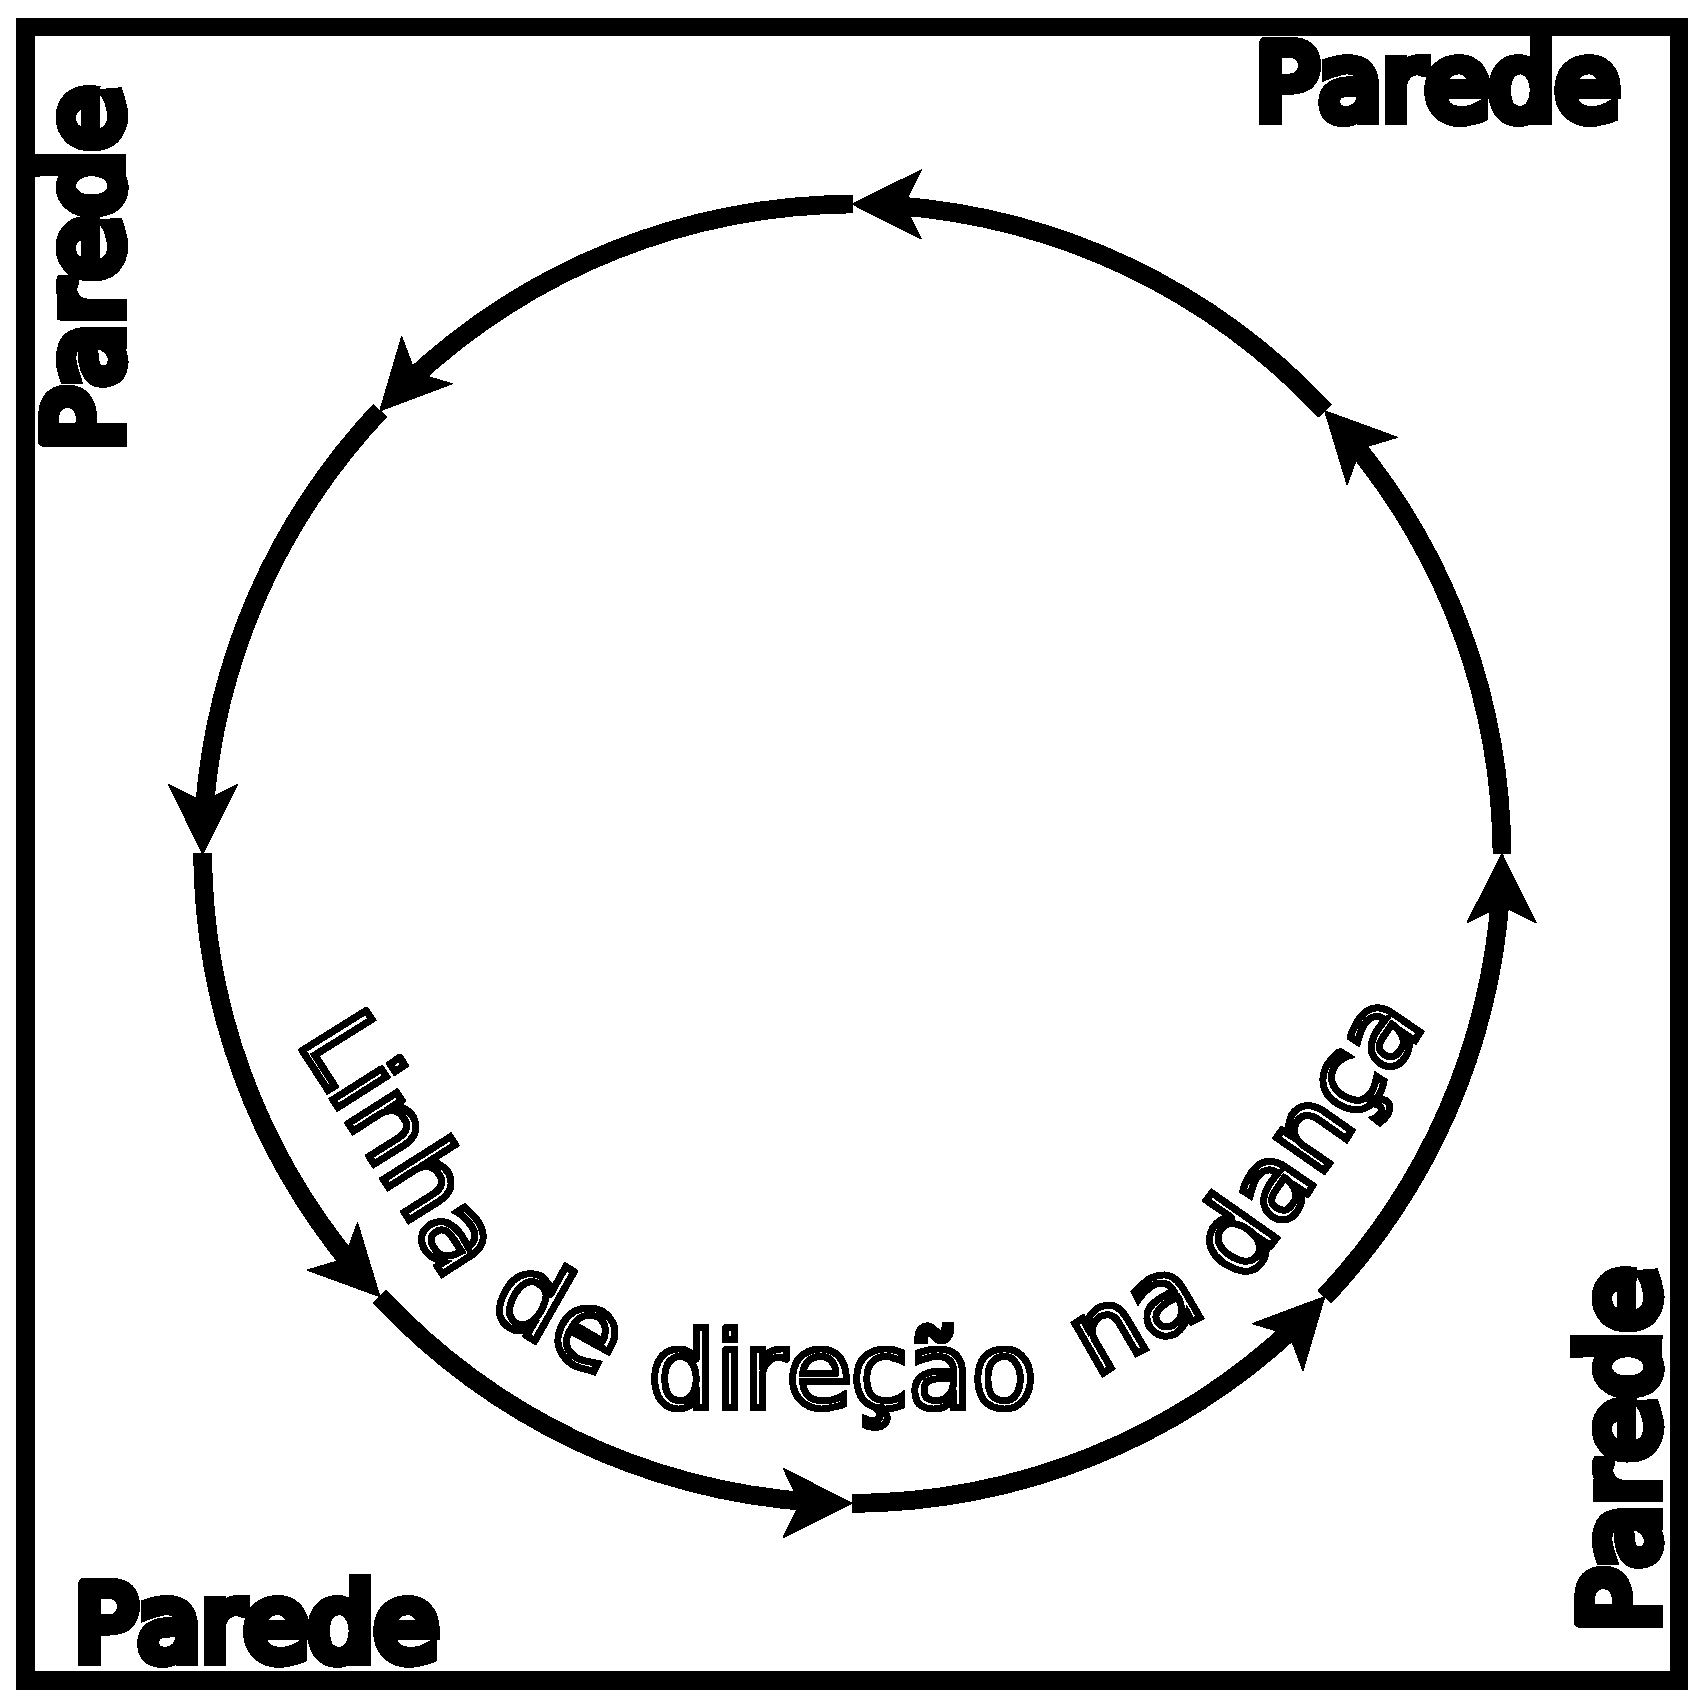
\includegraphics[width=0.3\textwidth]{chapters/cap-normas/circular-antihorario.eps}
\caption{Linha de direção nas danças com  deslocamento circular \cite[pp. 20]{freitas1959danca}.}
\label{fig:giro-antihorario1}
\end{figure}
Visto o anterior é importante ressaltar que né todas as danças tem
uma evolução circular na pista de dança, pois existem estilos de dança que são dançados em linha,
como por exemplo a ``Salsa em linha'' ou o ``West coast swing''; ou também existem estilos que
tem um comportamento hibrido entre circular e linha como o "Zouk". Neste sentido,
a ``samba de gafieira'' tem um comportamento circular e  deve ser dançado
rodando o salão para um boa etiqueta na pista de dança.


\item[Conduzir e ser conduzidos:] Trabalhar num \hyperref[def:ParadigmaConducao]{\textbf{paradigma da dança baseado
na condução}} é muito importante para na \hyperref[def:DancaSalao]{\textbf{dança de salão}}, dado que isto implicará
que um \hyperref[def:Condutor]{\textbf{condutor}} habilidoso, poderá dançar fluidamente com pessoas com quem nunca dançou
antes (se esta for conduzível). De forma similar acontecerá para os \hyperref[def:Seguidor]{\textbf{seguidores}} que desenvolvam
a sensibilidade necessária para serem conduzíveis, elas poderão dançar com qualquer
condutor, inclusive poderão ter um desenvolvimento básico em estilos de dança pouco ou não conhecidos.

O caso oposto ao \hyperref[def:ParadigmaConducao]{\textbf{paradigma da condução}}, é ter um estilo de dança baseado em coreografias;
este enfoque, dependendo da finalidade, pode ser visto como um vicio que geralmente aparece quando iniciamos
na dança. 
\begin{example}[Dançando de forma coreográfica:]
Quando a pessoa que deve conduzir, assume que se esta realiza só a parte do movimento 
que lhe corresponde, sem enviar nenhuma informação ao \hyperref[def:Par]{\textbf{par}}, 
o \hyperref[def:Seguidor]{\textbf{seguidor}} deve reconhecer/adivinhar o movimento que o condutor imaginou.
\end{example} 
O enfoque do exemplo anterior, funciona bem quando ambos dançarinos tem treinado antecipadamente os movimentos, 
e/ou conhecem a sequencia em que estes movimentos serão executados; 
porem, falha quando os dançarinos não se conhecem.
Comprovar isto é fácil se imaginamos, por exemplo, o caso em que o \hyperref[def:Condutor]{\textbf{condutor}} executa um movimento
que tem a parte inicial muito parecida a outro movimento, nesse caso, se o \hyperref[def:Seguidor]{\textbf{seguidor}} não tiver
um poder telepático confundirá um movimento com o outro e acontecerá um problema de comunicação. Assim, a coreografia
na dança deve estar reservada para apresentações, onde o \hyperref[def:Par]{\textbf{par}} volta 
a sua atenção para a encenação da peça, e não para detalhes mais mecânicos.

\item[Peso do corpo definido num pé:] Em estilos de dança onde uma boa postura é requerida,
ter o peso total do corpo bem definido sobre um pé, 
ao final de cada ação ou proposta de movimento,
quando sabemos que realizaremos mais movimentos imediatamente depois;
garante conservar a postura e ter uma maior velocidade no tempo de reação para o seguinte movimento;
pois, ao ter um pé livre poderemos mover ele sem temor a perder o equilibro, 
o que se traduz na leveza na execução dos movimentos. 
Isto é facilmente comprovável se fazemos um pequeno exercício. 
\begin{example}
Ao ficar em pé separamos as
pernas uma distancia igual à de nosso quadril, e nesse momento levamos o peso do corpo\footnote{
Em física podemos representar um corpo como um objeto com a masa concentrada no seu centro de gravidade, 
que no casso do ser humano está perto do umbigo.} a
apontar a um ponto médio entre nossos pés, nesse instante estamos dividindo o peso do corpo
entre nossos dois pontos de apoio, 50$\%$ no pé direito e 50$\%$ no pé esquerdo; agora, mantendo o peso
do corpo nesse lugar, tentaremos levantar qualquer de nossos pés, será evidente
que esse trabalho é muito difícil sem perder o equilíbrio, pois para mantê-lo
precisamos de ambos pontos de apoio; casos similares podem ser vistos com qualquer proporção de distribuição de peso,
por exemplo, 30$\%$ e 70$\%$ ou 20$\%$ e 80$\%$. 
\end{example}
Assim, do exemplo anterior se deduz, que estaremos
equilibrados, e poderemos executar nossos movimentos e levantar um pé 
mantendo a postura e auto controle, quando
temos o 100$\%$ do peso do corpo num pé só, o pé de apoio.
 
Por outro lado, quando consideramos ao 
\hyperref[def:Condutor]{\textbf{condutor}} como o agente desequilibrante do \hyperref[def:Seguidor]{\textbf{seguidor}}, 
por exemplo no caso em que este aplica uma condução;
a ideia de manter o peso do corpo num pé só, tem um valor agregado; 
pois fica mais fácil para o condutor orientar
ao seguidor a fazer o seguinte movimento, dado que o único pé que o seguidor pode mover é o pé
que está livre, e que é o pé que o condutor precisa que se movimente, 
além de que a força necessária pelo condutor para tirar ao seguidor do seu equilíbrio 
atual é muito menor ao caso quando o seguidor tem dois pontos de apoio.
Adicionalmente o seguidor tem um pé livre para se resguardar do desequilíbrio, provocado pelo 
condutor, e adquirir um novo equilíbrio com esse pé.

Outra forma equivalente de descrever, a localização do peso do corpo, 
é indicar que o peso do corpo deve recair sobre o pé que está em frente, 
quando realizamos um passo de avanço, 
e no pé que está atrás quando realizamos passos de recuo \cite[pp. 19]{freitas1959danca}.


\textbf{Nunca podemos dividir o peso do corpo?} Esta caraterística é possível sim,
se nossa dança fosse um relato escrito, o peso de nosso corpo deve estar bem definido num pé,
ao final de cada palavra, em cada virgula e ponto e virgula; por outra lado, 
o peso do corpo pode estar dividido em cada ponto.

\textbf{Este é o único meio de manter o equilíbrio na dança?}  Não, 
existem estilos de dança, como por exemplo no ``lindy hop'' onde se consegue manter os pês libres, 
para executar os movimentos, mantendo um equilíbrio dinâmico,
realizando um movimento de rebote (chamado ``bouncing'') ao ritmo da música.
O movimento consiste em deixar cair nosso corpo, flexionando ligeiramente  os joelhos, 
e imediatamente volver a ficar em pé, realizando assim um efeito de mola. 

\item[Ter uma boa conexão entre o par na dança:] Seguindo a ideia da condução, esta só pode
ser realizada se existe um médio de comunicação, onde possa ser transmitido
o comando do \hyperref[def:Condutor]{\textbf{condutor}} ao \hyperref[def:Seguidor]{\textbf{seguidor}}. 
Assim, um boa conexão garante este fluxo de informação entre o \hyperref[def:Par]{\textbf{par}} na dança. 
A forma exata de obter esta conexão varia ligeiramente entre os diferentes estilos de dança;
dado que em alguns casos será usado um \hyperref[def:abracodedanca]{\textbf{abraço de dança}} 
e em outros o par estará conectado segurando-se das mãos.
Mas, em todos os casos, 
o que se procurará é ter a maior quantidade de pontos de contato no par,
pois quanto mais pontos de contato tenhamos, 
maior será a fidelidade com que a informação da condução chegue ao seguidor.


Outro ponto importante desta conexão é a \hyperref[def:brazosfirmes]{\textbf{firmeza dos braços}}, 
pois é a traves deles que passa a maior parte da informação.
Assim, no caso do seguidor, ter os braços firmes implicará que qualquer informação que chegue por eles,
se transmitirá maioritariamente ao corpo,
mudando assim este de estado ou posição.

Em estilos de dança onde existe a possibilidade de dançar tomados das mãos,
se não se tem bem treinados os braços,
é muito fácil que a informação da condução seja perdida.
Isto acontece, porque no braço todo, temos vários graus de liberdade nas articulações.
Se algum destes pontos não tem a firmeza necessária para transportar a informação de condução, 
sem modificar maioritariamente sua posição relativa e postura,  
então esse ponto provocará a perdida da informação, 
pois se modificará a posição dos braços sem alterar a posição do corpo.
\begin{example}
De pie frente a frente com seu par, testaremos 3 formas de conduzir, 
criadas quando o condutor segura com as mãos ao seguidor, em 3 lugares diferentes:
\begin{itemize}
\item Segurando num ponto meio entre entre o cotovelo e os ombros,
\item segurando no antebraço, e
\item tomados das mãos.
\end{itemize}
\end{example}
No exemplo anterior, será muito evidente em seguidores iniciantes,
que a maior eficacia na transmissão de informação se consegue segurando entre os cotovelos e os ombros,
seguido por segurar pelo antebraço, e finalmente nas mãos;
é dizer, a eficacia na transmissão da informação, 
diminuí com o aumento dos grãos de liberdade.

Assim, para obter uma boa conexão no par, 
e eficacia na transmissão de informação, devemos ter:
\begin{itemize}
\item Uma boa postura de braços e
\item procurar a maior quantidade de pontos de contato.
\end{itemize}  

\end{description}
